\documentclass[xcolor=table]{beamer}

\setbeamerfont{title}{size=\LARGE}

% Logo
%\addtobeamertemplate{title page}{%
%  \begin{textblock}{20}(11.5,-0.5)%
%    \includegraphics[height=1in]{figures/white-logo}%
%  \end{textblock}%
%}

\usepackage[T1]{fontenc}
%\usepackage[sfdefault]{AlegreyaSans} %% Option 'black' gives heavier bold face
%% The 'sfdefault' option to make the base font sans serif
%\renewcommand*\oldstylenums[1]{{\AlegreyaSansOsF #1}}

\usepackage[scaled=0.85]{beramono}
\setbeamertemplate{navigation symbols}{} % strip navigation symbols
%\usefonttheme{serif} % use the sans-serif fonts (Palatino)
\setbeamerfont{title}{series=\bfseries,parent=structure}
\setbeamerfont{frametitle}{series=\bfseries,parent=structure}

\usepackage{textpos}
%\usepackage{paralist}
%\usepackage{enumitem}
\usepackage{expdlist}
\usepackage{subfigure}
\usepackage{amssymb, amsmath, amsthm}
\everymath{\displaystyle}

\usepackage[T1]{fontenc}
\usepackage{mathpazo}

\definecolor{mgcolor}{RGB}{230,230,230}
\definecolor{bgcolor}{RGB}{255,255,255}
\definecolor{fgcolor}{RGB}{0,0,0}

\newcommand{\code}[1]{\texttt{#1}}
\newcommand{\mono}[1]{\texttt{#1}}
\newcommand{\textt}[1]{\ensuremath{\text{\mono{#1}}}}
\newcommand{\mathmono}[1]{\ensuremath{\text{\mono{#1}}}}
\newcommand{\nonterm}[1]{\ensuremath{\text{\mono{<#1>}}}}
\newcommand{\term}[1]{\ensuremath{\text{\mono{`#1'}}}}
\newcommand{\any}[0]{\ensuremath{\left\langle\bigtriangleup\right\rangle}}
\newcommand{\D}{$\Delta$}

\newcommand{\makeTable}[6][htbp!]
{
	\begin{table}[#1]
	\centering
	\begin{tabular}{#4}
	#5\\
	#6\\
	\end{tabular}
	\end{table}
}

\newcommand{\includeFigure}[4][htbp!]
{
	\begin{figure}[#4]
	\centering
	\IfDecimal{#1}
	{
		\includegraphics[scale=#1]{figures/#2}
	}
	{
		\includegraphics[#1]{figures/#2}
	}
	\caption[]{#3}
	\label{figure:#2}
	\end{figure}
}

\usepackage{clrscode3e}
\usepackage{verbatim}
\usepackage{listings}
\lstset
{
  language=bash,
	tabsize=2,
	numbers=none,
	breaklines=true,
  backgroundcolor=\color{mgcolor},
%	foregroundcolor=\color{bgcolor},
	framexleftmargin=0.05in,
	basicstyle=\ttfamily\footnotesize,
	numberstyle=\tiny,
%  keywordstyle=\color{green},
%	stringstyle=\color{red},
%	commentstyle=\color{ForestGreen},
  mathescape=true,
  captionpos=t,
  columns=fullflexible,
  breakatwhitespace,
  extendedchars=true,
%  escapeinside={(*@}{@*)},
  mathescape=false,
  keepspaces,
  emphstyle={\bf},
  showstringspaces=false,
}

\setbeamercolor{title}{fg=fgcolor}
\setbeamercolor{frametitle}{fg=fgcolor}
\setbeamercolor{normal text}{fg=fgcolor}
\setbeamercolor{background canvas}{bg=bgcolor}
\setbeamercolor{normal text}{fg=fgcolor}
\setbeamercolor{itemize item}{fg=fgcolor}
\setbeamercolor{itemize subitem}{fg=fgcolor}
\setbeamercolor{description item}{fg=fgcolor}
\setbeamercolor{enumerate item}{fg=fgcolor}
\setbeamercolor{block title}{fg=fgcolor}

\setbeamercolor{bibliography item}{fg=fgcolor}
\setbeamercolor{bibliography entry author}{fg=fgcolor}
%\setbeamertemplate{bibliography item}[text]

\usepackage{fancyvrb}

\newcommand{\question}[1]%
{%
  \begin{center}%
  \Large \textbf{#1}%
  \end{center}%
}

\newcommand{\answer}[1]%
{%
  \begin{flushright}%
  --- #1%
  \end{flushright}%
}

\usepackage{xparse}

\NewDocumentCommand\mathWrap{mmm}{\ensuremath{%
  \mathopen{}\left#1#2\right#3\mathclose{}%
}}

\NewDocumentCommand\set{m}{%
  \mathWrap{\{\mathrel{}}{#1\mathrel{}}{\}}%
}

\NewDocumentCommand\floor{m}{%
  \mathWrap{\lfloor\mathrel{}}{#1\mathrel{}}{\rfloor}%
}

\NewDocumentCommand\card{m}{%
  \mathWrap{|\mathrel{}}{#1\mathrel{}}{|}%
}

\NewDocumentCommand\p{m}{%
  \mathWrap{(}{#1}{)}%
}

\usepackage{bashful}

\usepackage{wasysym}

% This file was generated from an m4 template.
% Generation date-time (ISO 8601): 2019-03-10T10:14+00:00
% Git remote URL: https://github.com/emerald/modes-listings
% Git commit ID: 58c030135c5312f58537438e766054171f662ddf

% Copyright (c) 2019 Oleks <oleks@oleks.info>
% 
% Permission is hereby granted, free of charge, to any person obtaining
% a copy of this software and associated documentation files (the
% "Software"), to deal in the Software without restriction, including
% without limitation the rights to use, copy, modify, merge, publish,
% distribute, sublicense, and/or sell copies of the Software, and to
% permit persons to whom the Software is furnished to do so, subject to
% the following conditions:
% 
% The above copyright notice and this permission notice shall be
% included in all copies or substantial portions of the Software.
% 
% THE SOFTWARE IS PROVIDED "AS IS", WITHOUT WARRANTY OF ANY KIND,
% EXPRESS OR IMPLIED, INCLUDING BUT NOT LIMITED TO THE WARRANTIES OF
% MERCHANTABILITY, FITNESS FOR A PARTICULAR PURPOSE AND NONINFRINGEMENT.
% IN NO EVENT SHALL THE AUTHORS OR COPYRIGHT HOLDERS BE LIABLE FOR ANY
% CLAIM, DAMAGES OR OTHER LIABILITY, WHETHER IN AN ACTION OF CONTRACT,
% TORT OR OTHERWISE, ARISING FROM, OUT OF OR IN CONNECTION WITH THE
% SOFTWARE OR THE USE OR OTHER DEALINGS IN THE SOFTWARE.

\lstdefinelanguage{emerald}
{
 % Keywords and built-in types, as found in:
  % Git remote URL: https://github.com/emerald/old-emerald
  % Git commit ID: 8de69f56ed8a7dcec2aacae369d2a20f29dfe960
  morekeywords={
    accept, and, as, assert,
    at, attached, awaiting, begin,
    builtin, by, checkpoint, class,
    closure, codeof, const, else,
    elseif, end, enumeration, exit,
    export, external, failure, false,
    field, fix, for, forall,
    from, function, if, immutable,
    in, initially, isfixed, islocal,
    locate, loop, monitor, move,
    nameof, new, nil, object,
    op, operation, or, primitive,
    process, record, recovery, refix,
    restrict, return, returnandfail, self,
    signal, suchthat, syntactictypeof, then,
    to, true, typeobject, typeof,
    unavailable, unfix, var, view,
    visit, wait, when, while, where
  },
  moreemph={
    Any, AOpVecE, AOpVec, AParamL,
    Array, AType, Bitchunk, Boolean,
    Buffer, Char, Cond, COpVecE,
    COpVec, CType, Decoder, Direct,
    GroupBase, Group, Handler, InStr,
    Integer, IState, IVec, IVOfAny,
    IVOfInt, IVOfStr, Literal, Makefile,
    name, new_Integer, Nil, NLElem,
    NodeL, Node, OutStr, RDirect,
    Real, realNode, RISA, RISC,
    Sequence, Signat, String, Stub,
    Time, Unix, vec-ed, vec-ed,
    Vec, VOfAny, VOfChar, VOfInt,
    VOfStr, xReal, xxxLiteral, 
  },
  % The other parts of the syntax spec, as found in other.vim:
  sensitive = false,
  morecomment=[l]{\%},
  morestring=[b]",
  morestring=[b]',
}

\lstset{language=emerald}

\title{{\Large Lecture 2: Emerald Objects and Types}}
\subtitle{An OO Language for Distributed Applications}
\subject{IN59570: Distributed Objects}
\institute{University of Oslo}
\author{Oleks Shturmov\\[-0.2em]%
  {\tiny \texttt{<olekss@uio.no>} / \texttt{<oleks@oleks.info>}}
}
\date{January 31, 2019\\[2em]
{\scriptsize Lecture slides derived from the 2018 lectures slides by%
Eric Jul: \\ {\tiny%
\url{https://www.uio.no/studier/emner/matnat/ifi/INF5510/v18/lectures-v18/f2/}}%
\\[1em] The source code for these slides is maintained here: \\[-0.5em] {\tiny%
\url{https://github.com/emerald/in5570v19/tree/master/lectures/2}}%
}}

\newcommand\inputsrc[1]{\lstinputlisting{../emerald/#1}}

\begin{document}

\begin{frame} \titlepage \end{frame}

\begin{frame}[fragile]

\frametitle{The People Behind Emerald}

\footnotesize
\def\arraystretch{1.5}

\begin{itemize}

\item Work done at the University of Washington in the early to mid-1980s

\item See HOPL paper for more details on the history of
Emerald\footnote{{\tiny
\url{https://www.uio.no/studier/emner/matnat/ifi/INF5510/v16/material/emerald-hopl.pdf}}}

\end{itemize}
\vspace{-1.2em}
\begin{table}
\centering
\begin{tabular}{rcc}
& \textbf{Runtime and Mobility} & \textbf{Language Design} \\\hline
\textbf{PhD Students} & %
\begin{minipage}{10em}%
\begin{center}%
\raisebox{-1.1\totalheight}{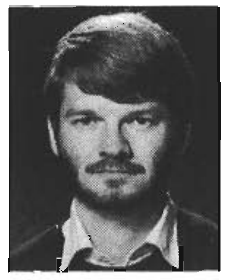
\includegraphics[width=0.5\textwidth]{figures/eric}}\\%
Eric Jul\\[1em]%
\end{center}%
\end{minipage} %
\footnote{{\tiny Today, Professor at the University of Oslo}}%
& %
\begin{minipage}{10em}%
\begin{center}%
\raisebox{-1.1\totalheight}{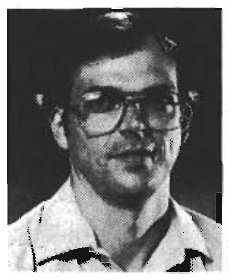
\includegraphics[width=0.5\textwidth]{figures/norman}}\\%
Norm Hutchinson%
\end{center}%
\end{minipage} %
\footnote{{\tiny Today, Associate Professor at the University of British Columbia}}%
\\
\textbf{Faculty} & %
\begin{minipage}{10em}%
\begin{center}%
\raisebox{-1.1\totalheight}{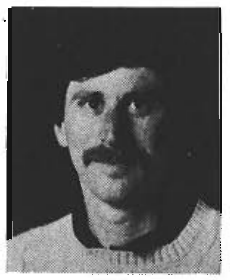
\includegraphics[width=0.5\textwidth]{figures/henry}}\\%
Hank Levy
\end{center}%
\end{minipage}%
\footnote{{\tiny Today, Chair in Computer
Science \& Engineering at the University of Washington}}%
& %
\begin{minipage}{10em}%
\begin{center}%
\raisebox{-1.1\totalheight}{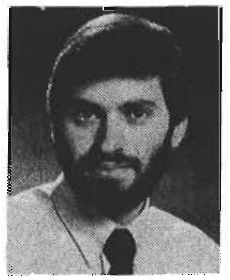
\includegraphics[width=0.5\textwidth]{figures/andrew}}\\%
Andrew Black%
\end{center}%
\end{minipage} %
\footnote{{\tiny Today, Professor at Portland State University}}%
\end{tabular}
\end{table}

\end{frame}


\begin{frame}

\frametitle{Principle: Everything Is an Object\footnote{Well, almost
everything}}

\begin{itemize}

\item Basic types (integers, booleans, strings, etc.) are objects

\item Classes are objects (in Emerald, mere syntactic sugar)

\item Types are objects (of a special built-in type, \texttt{Signature})

\item Language constructs however, are \textbf{\underline{not}}
objects \\ (e.g., declarations, if-statements, for-loops, programs)

\end{itemize}

\vspace{\fill}

\textbf{Alternative interpretation:}

Every valid expression evaluates to an object

\vspace{\fill}

Consequently:

\begin{itemize}

\item Type names and declarations are expressions

\item Class names and declarations are expressions

\end{itemize}

\end{frame}

% \begin{frame}
% 
% \frametitle{How Can You Test If Something Is An Object?}
% 
% \begin{itemize}
% 
% \item 
% 
% \end{itemize}
% 
% \end{frame}
% 
% 
% \begin{frame}
% 
% \frametitle{Classless Objects}
% 
% \begin{itemize}
% 
% \item In Emerald, defining an object type, and instantiting an object
% of that type are done in one go.
% 
% \end{itemize}
% 
% \end{frame}


\begin{frame}[fragile]

\frametitle{Some Non-Objects: Trivial Emerald Programs}

\begin{itemize}

\item An Emerald program is a list of constant declarations

\item Each bearing a name, an expression, and optionally, a type

\item The following (trivial) programs produce no output

\end{itemize}

With type inference:

\inputsrc{00-trivial-type-inference.m}

With type annotations:

\inputsrc{01-trivial-type-annotations.m}

\end{frame}


\begin{frame}[fragile]

\frametitle{Some Hello-World Objects (1/3)}

Time for some output!

\lstinputlisting{../src/02-hello-world.m}

To compile and run:

\begin{lstlisting}
$ ec hello.m    # Assuming you call the above file hello.m
$ emx hello.x   # Assuming ec went well, you'll get a hello.x
\end{lstlisting}

\begin{itemize}

\item The use of the name(s) ``\texttt{main}'' is purely conventional

\item Emerald merely evaluates the declarations of a program\\ (and
their expressions) in order, from top to bottom

\item An \texttt{initially}-block can contain a list of declarations
and statements, and end in fault-handling code; more on fault-handling
in subsequent lectures

\end{itemize}

\end{frame}

\begin{frame}[fragile]

\frametitle{Some Hello-World Objects (2/3)}

The following is also a valid Emerald program:

\lstinputlisting{../src/03-alice-bob-say-hello.m}

Compile and run:

\begin{lstlisting}
$ ec hello.m
$ emx hello.x
Hello, I am Alice!
Hello, I am Bob!
\end{lstlisting}

\end{frame}

\begin{frame}[fragile]

\frametitle{Some Hello-World Objects (3/3)}

So is this:

\lstinputlisting{../src/04-lonely-planet.m}

Compile and run:

\begin{lstlisting}
$ ec hello.m
$ emx hello.x
Hello, World!
Hello?
Is there anyone out there?
\end{lstlisting}

\end{frame}


\begin{frame}[fragile]

\frametitle{A More Elaborate Object (1/3)}

\begin{lstlisting}
% A random number generator
% Derived from https://stackoverflow.com/a/3062783/5801152
const rand <- object rand
  var seed : Integer <- 123456789
  const a <- 1103515245
  const c <- 12345
  const m <- 2147483648
  op next -> [retval : Integer]
    seed <- (a * seed + c) # m
    retval <- seed
  end next
  initially
    stdout.putstring[rand.next.asstring || "\n"]
    stdout.putstring[rand.next.asstring || "\n"]
    stdout.putstring[rand.next.asstring || "\n"]
  end initially
end rand
\end{lstlisting}

\begin{itemize}

\item Many built-in types define an \texttt{asstring} method

\item Append a line break (\lstinline{|| "\n"}) to flush stdout

\end{itemize}

\end{frame}

\begin{frame}[fragile]

\frametitle{A More Elaborate Object (2/3)}

If we \textbf{export} the operation, we can use it outside:

\begin{lstlisting}
const rand <- object rand
  var seed : Integer <- 123456789
  const a <- 1103515245
  const c <- 12345
  const m <- 2147483648
  export op next -> [retval : Integer]       % See here
    seed <- (a * seed + c) # m
    retval <- seed
  end next
end rand                                    % Here
                                            %
const main <- object main                   %
  initially
    stdout.putstring[rand.next.asstring || "\n"]
    stdout.putstring[rand.next.asstring || "\n"]
    stdout.putstring[rand.next.asstring || "\n"]
  end initially
end main                                    % And here
\end{lstlisting}

\end{frame}


\begin{frame}[fragile]

\frametitle{A More Elaborate Object (3/3)}

Now, with a bit more \textbf{class}:

\begin{lstlisting}
const rand <- class rand                  % See here
  var seed : Integer <- 123456789
  const a <- 1103515245
  const c <- 12345
  const m <- 2147483648
  export op next -> [retval : Integer]
    seed <- (a * seed + c) # m
    retval <- seed
  end next
end rand

const main <- object main
  initially
    const r <- rand.create                % And here
    stdout.putstring[r.next.asstring || "\n"]
    stdout.putstring[r.next.asstring || "\n"]
    stdout.putstring[r.next.asstring || "\n"]
  end initially
end main
\end{lstlisting}

\end{frame}


\begin{frame}[fragile]

\frametitle{What Is A Class (in Emerald) Anyway?}

\begin{center}

A class declares (1) an object type, and \\ (2) a means to create
instances of that type

\end{center}

\vspace{\fill}

Consequently, an Emerald class \texttt{C} is
\textbf{\underline{syntactic sugar}}\\ for an Emerald object exporting
the following methods:

\begin{lstlisting}
getSignature -> Signature
create [p1, p2, ...] -> C
\end{lstlisting}

where

\begin{itemize}

\item \lstinline{Signature} is a built-in type of all type objects

\item The value (object) returned by \texttt{create} will ``conform
to''\\ the signature returned by \texttt{getSignature}

\end{itemize}

More on type objects and conformity after an example

\end{frame}

\begin{frame}[fragile]

\frametitle{A More Elaborate (Class) Object}

The class from before, without syntactic sugar:

\begin{lstlisting}
const rand <- object RandCreator
  const RandType <- typeobject RandType
    op next -> [seed : Integer]
  end RandType
  export function getSignature -> [r : Signature]
    r <- RandType
  end getSignature
  export op create -> [r : RandType]
    r <- object Rand
      var seed : Integer <- 123456789
      const a <- 1103515245
      const c <- 12345
      const m <- 2147483648
      export operation next[] -> [r : Integer]
        seed <- (a * seed + c) # m
        r <- seed
      end next
    end Rand
  end create
end RandCreator
\end{lstlisting}

\end{frame}



\begin{frame}

\frametitle{Type Objects}

\begin{itemize}

\item Special objects of the built-in type \lstinline{Signature}

\item Constructed using the \lstinline{typeobject} keyword

\item Every Emerald object has an associated type object

\item Use the \lstinline{typeof} operator to fetch the type of an object

\item Use the \lstinline{getSignature} method to fetch the type of a class

\item Compare type objects with the \lstinline{*>} (conforms to)
operator

\end{itemize}

\end{frame}

\begin{frame}[fragile]

\frametitle{Type Objects: Examples (1/3)}

\inputsrc{09-typeof-conforms-to.m}

\end{frame}

\begin{frame}[fragile]

\frametitle{Type Objects: Examples (2/3)}

\inputsrc{10-getSignature-conforms-to.m}

\end{frame}

\begin{frame}[fragile]

\frametitle{Type Objects: Examples (3/3)}

\inputsrc{11-typeof-conforms-to-getSignature.m}

\end{frame}


\begin{frame}[fragile]

\frametitle{Type Conformity Is Everywhere}

\begin{center}

When using an object where a particular type is expected,\\ the object
type must \textbf{\underline{conform to}} the expected type

\end{center}

\begin{itemize}

\item Conformity is checked at compile time; no runtime costs!

\end{itemize}

\inputsrc{12-instance-conforms-to-type.m}

\end{frame}


\begin{frame}[fragile]

\frametitle{Type Conformity: Definition}

\newcommand{\emlbr}{\ensuremath{\text{\texttt{[}}}}
\newcommand{\emrbr}{\ensuremath{\text{\texttt{]}}}}
\newcommand{\emrarr}{\ensuremath{\text{\texttt{->}}}}
\newcommand{\emsig}[3]{\ensuremath{#1\emlbr {#2}\emrbr\emrarr\emlbr {#3}\emrbr}}

A type $S$ conforms to a type $T$ iff for each operation

$$\emsig{o}{p^T_1, p^T_2, \ldots p^T_n}{r^T_1, r^T_2, \ldots,
r^T_m}\quad \text{in}\ T$$

there is a corresponding operation\footnote{Having the same name,
number of formal parameters, and results.}

$$\emsig{o}{p^S_1, p^S_2, \ldots p^S_n}{r^S_1, r^S_2, \ldots,
r^S_m}\quad \text{in}\ S$$

where

\begin{enumerate}

\item $p^T_i$ conforms to $p^S_i$, for all $i \in 1, 2, \ldots n$, and

\item $r^S_i$ conforms to $r^T_i$, for all $i \in 1, 2, \ldots n$

\end{enumerate}

\vspace{\fill}

\begin{center}

NB! Formal parameters conform one way, while results the other.

\end{center}

\end{frame}


\begin{frame}

\frametitle{Some Special Cases: Any and None}

\begin{center}

\lstinline{Any} and \lstinline{None} are special built-in types

\lstinline{None} is the type of the keyword (expression) \lstinline{nil}

\end{center}

\vspace{\fill}

They have the following interesting properties:

\begin{enumerate}

\item Everything conforms to \lstinline{Any}

\item \lstinline{None} conforms to anything

\item Nothing conforms to \lstinline{None}

\end{enumerate}

Notably, \lstinline{nil} conforms to \lstinline{Any}, and anything at all

\end{frame}


\begin{frame}[fragile]

\frametitle{Type Conformity: Example (1/3)}

Consider the types of some waste bins, which we can pick at:

\begin{center}
\begin{minipage}{0.4\textwidth}
\begin{lstlisting}
typeobject AnyBin
  op Pick -> [Any]
end AnyBin
\end{lstlisting}
\end{minipage}\quad%
\begin{minipage}{0.4\textwidth}
\begin{lstlisting}
typeobject PaperBin
  op Pick -> [Paper]
end PaperBin
\end{lstlisting}
\end{minipage}
\end{center}

Now, imagine being a waste picker\footnote{Waste-picking is an
admirable profession for an autonomous drone}:

\begin{itemize}

\item If you accept any trash (i.e., \texttt{AnyBin}s), then you are
also willing accept specialized trash (e.g., \texttt{PaperBin}s).

\item If you only accept specialized trash (e.g., \texttt{PaperBin}s),
then you are not willing to accept any trash (i.e., \texttt{AnyBin}s).

\end{itemize}

Hence, \texttt{PaperBin} conforms to \texttt{AnyBin}, but not
vice-versa.

\end{frame}


\begin{frame}[fragile]

\frametitle{Type Conformity: Example (2/3)}

Now, instead consider bins we can throw something into:

\begin{center}
\begin{minipage}{0.4\textwidth}
\begin{lstlisting}
typeobject AnyBin
  op Throw[Any]
end AnyBin
\end{lstlisting}
\end{minipage}\quad%
\begin{minipage}{0.4\textwidth}
\begin{lstlisting}
typeobject PaperBin
  op Throw[Paper]
end PaperBin
\end{lstlisting}
\end{minipage}
\end{center}

\begin{itemize}

\item A bin that accepts anything (i.e., \texttt{AnyBin}), can\\ also
act as a specialized bin (e.g., \texttt{PaperBin}).

\item A specialized bin however (e.g., \texttt{PaperBin}), cannot\\
act as a bin for anything (i.e., \texttt{AnyBin}).

\end{itemize}

Hence, \texttt{AnyBin} conforms to \texttt{PaperBin}, but not vice-versa.

\end{frame}

\begin{frame}[fragile]

\frametitle{Type Conformity: Example (3/3)}

Combining the two examples however, yields non-conforming bins:

\begin{center}
\begin{minipage}{0.4\textwidth}
\begin{lstlisting}
typeobject AnyBin
  op Pick -> [Any]
  op Throw[Any]
end AnyBin
\end{lstlisting}
\end{minipage}\quad%
\begin{minipage}{0.4\textwidth}
\begin{lstlisting}
typeobject PaperBin
  op Pick -> [Paper]
  op Throw[Paper]
end PaperBin
\end{lstlisting}
\end{minipage}
\end{center}

This makes sense:

\begin{itemize}

\item You cannot throw anything into a \texttt{PaperBin},\\ so it
cannot act as an \texttt{AnyBin}.

\item You can throw anything into an \texttt{AnyBin}, so it cannot act
as a \texttt{PaperBin}, from which you only ever want to pick
\texttt{Paper}.

\end{itemize}

Hence, neither \texttt{AnyBin} conforms to \texttt{PaperBin}, nor
vice-versa.

\end{frame}


\begin{frame}

\frametitle{Further Reading}

\begin{thebibliography}{Dijkstra, 1982}

\bibitem[Raj et al., 1991]{report1991} Raj, Tempero, Levy, Black,
Hutchinson, and Jul (1991), Technical Report: The Emerald Programming
Language\\ {\tiny
\url{https://www.uio.no/studier/emner/matnat/ifi/INF5510/v15/pensum/Report.pdf}}

\end{thebibliography}
\end{frame}


\end{document}
